%%%%%%%%%%%%%%%%%%%%%%%%%%%%%%%%%%%%%%%%%%%%%%%%%%%%%%%%%%%%%%%%%%%%
%% I, the copyright holder of this work, release this work into the
%% public domain. This applies worldwide. In some countries this may
%% not be legally possible; if so: I grant anyone the right to use
%% this work for any purpose, without any conditions, unless such
%% conditions are required by law.
%%%%%%%%%%%%%%%%%%%%%%%%%%%%%%%%%%%%%%%%%%%%%%%%%%%%%%%%%%%%%%%%%%%%

\newif\iftodo
% Enable todo notes in the margins.
% \todotrue

\newif\ifexamples
% \examplestrue

\documentclass[
  digital,     %% The `digital` option enables the default options for the
               %% digital version of a document. Replace with `printed`
               %% to enable the default options for the printed version
               %% of a document.
%%  color,       %% Uncomment these lines (by removing the %% at the
%%               %% beginning) to use color in the printed version of your
%%               %% document
  oneside,     %% The `oneside` option enables one-sided typesetting,
               %% which is preferred if you are only going to submit a
               %% digital version of your thesis. Replace with `twoside`
               %% for double-sided typesetting if you are planning to
               %% also print your thesis. For double-sided typesetting,
               %% use at least 120 g/m² paper to prevent show-through.
  nosansbold,  %% The `nosansbold` option prevents the use of the
               %% sans-serif type face for bold text. Replace with
               %% `sansbold` to use sans-serif type face for bold text.
  nocolorbold, %% The `nocolorbold` option disables the usage of the
               %% blue color for bold text, instead using black. Replace
               %% with `colorbold` to use blue for bold text.
  lof,         %% The `lof` option prints the List of Figures. Replace
               %% with `nolof` to hide the List of Figures.
  nolot,       %% The `lot` option prints the List of Tables. Replace
               %% with `nolot` to hide the List of Tables.
]{fithesis4}
%% The following section sets up the locales used in the thesis.
\thesissetup{
    date        = \the\year/\the\month/\the\day,
    university  = mu,
    faculty     = fi,
    type        = bc,
    department  = Department of Machine Learning and Data Processing,
    author      = Dominik Rehák,
    gender      = m,
    advisor     = {RNDr. Vít Novotný, Ph.D.},
    title       = {Generic TeX Writer for the Pandoc Document Converter},
    TeXtitle    = {Generic \TeX{} Writer for the Pandoc Document Converter},
    keywords    = {TeX, LaTeX, Markdown, Pandoc, Lua, text analysis and parsing},
    TeXkeywords = {\TeX{}, \LaTeX{}, Markdown, Pandoc, Lua, text analysis and parsing},
    abstract    = {%
      Pandoc is a utility able to convert between dozens of document formats
      including \TeX{} formats such as \LaTeX{} and Con\TeX{}t, but it provides
      no support for other well-known \TeX{} formats such as plain \TeX{}.
      Moreover, it offers no way to influence the style of its output. The goal
      of this thesis is to integrate Pandoc with the \TeX{} package Markdown,
      which allows users to embed blocks of text in the lightweight markup
      language Markdown into their documents, as well as change the styling of
      individual elements. Using macros from the Markdown package, the author
      produces a proof of concept for a generic \TeX{} writer for Pandoc, which
      is also capable of producing output for any \TeX{} format based on plain
      \TeX{}.
      \ifexamples
        Usage of the writer is then demonstrated on a set of example documents.
      \fi
    },
    thanks      = {%
      I would like to thank my supervisor, RNDr. Vít Novotný, Ph.D., for his
      unceasing guidance and support during the writing of this thesis. I would
      also like to thank my family, friends, coworkers and everyone else who
      hasn't given up on me during my studies and continued to offer unceasing
      love and encouragement.
    },
    bib         = bibliography.bib,
    %% Remove the following line to use the JVS 2018 faculty logo.
    facultyLogo = fithesis-fi,
}
%% These additional packages are used within the document:
\usepackage{paralist} %% Compact list environments
\usepackage{amsmath}  %% Mathematics
\usepackage{amsthm}
\usepackage{amsfonts}
\usepackage{url}      %% Hyperlinks
\usepackage{markdown} %% Lightweight markup
\usepackage{multicol}
\usepackage[dvipsnames]{xcolor}
\usepackage{tikz}
\usetikzlibrary{positioning}
\usepackage{listings} %% Source code highlighting
\lstset{
  basicstyle      = \ttfamily,
  identifierstyle = \color{black},
  keywordstyle    = \color{blue},
  keywordstyle    = {[2]\color{cyan}},
  keywordstyle    = {[3]\color{olive}},
  stringstyle     = \color{teal},
  commentstyle    = \itshape\color{magenta},
  breaklines      = true,
  columns         = fullflexible,
  aboveskip       = 2em,
  belowskip       = 2em,
}
\usepackage{floatrow} %% Putting captions above tables
\floatsetup[table]{capposition=top}
% \usepackage[babel]{csquotes} %% Context-sensitive quotation marks
\usepackage{pdfpages}
\usepackage{graphicx}
\usepackage[export]{adjustbox}
\iftodo
  \usepackage[backgroundcolor=Apricot,linecolor=Apricot]{todonotes}
\else
  \usepackage[disable]{todonotes}
\fi

\usepackage{microtype}
\usepackage{hyphenat}
\usepackage[T1]{fontenc}
\hyphenation{light-weight}
\hyphenation{con-struc-tors}
\hyphenation{Čes-ko-slo-ven-ské-ho}

\newcommand\macro[1]{\texttt{\textbackslash{}{#1}}}
\newcommand\pandoc[1]{\macro{pandoc\-{#1}}}
\newcommand\renderer[1]{\macro{markdown\-Renderer\-{#1}}}
\ExplSyntaxOn
\newcommand\file[1]
  {
    \str_case:nn
      { #1 }
      {
        { p2md.lua } { \texttt{pandoc\hyp{}to\hyp{}markdown.lua} }
        { p2md.tex } { \texttt{pandoc\hyp{}to\hyp{}markdown.tex} }
        { p2md.sty } { \texttt{pandoc\hyp{}to\hyp{}markdown.sty} }
        % TODO add default
      }
  }
\ExplSyntaxOff

\begin{document}
%% Uncomment the following lines (by removing the %% at the beginning)
%% and to print out List of Abbreviations and/or Glossary in your
%% document. Titles for these tables can be changed by replacing the
%% titles `Abbreviations` and `Glossary`, respectively.
%% \clearpage
%% \printnoidxglossary[title={Abbreviations}, type=\acronymtype]
%% \printnoidxglossary[title={Glossary}]

\chapter{Introduction}
\TeX{} is a digital typesetting system capable of producing high-quality documents. It is especially widespread in academia because of its abilities in the typesetting of mathematics. However, its language can be verbose and cryptic for new and inexperienced users. The Markdown package addresses this by allowing users to supplement their \TeX{} documents with blocks of text written in Markdown, a markup language that is widespread on the Internet and easy to read and write.

Pandoc is a utility able to convert between numerous document formats, including HTML, Markdown, or \LaTeX{} and Con\TeX{}t, two popular formats of \TeX{}. However, Pandoc does not provide a way to redefine the style of its output without reprogramming and recompiling Pandoc itself. It is true that the output can be edited further, but repeated conversion would undo such edits. Moreover, Pandoc does not provide a way to output documents for plain \TeX{} (i.e. without \LaTeX{} or Con\TeX{}t on top).

The goal of this thesis is to integrate Pandoc with the Markdown package. Such an integration would allow users to supplement their \TeX{} documents with other documents or document snippets in formats such as HTML, DOCX or RTF. Moreover, since the Markdown package is capable of plain \TeX{} output, this would provide a way to obtain plain \TeX{} output from Pandoc.

In Chapter 2, the author introduces Pandoc, \TeX{} and the Markdown package and outlines the proof of concept of the integration. Chapter 3 describes this proof of concept in greater
\ifexamples
  detail and Chapter 4 demonstrates its practical usage on a set of example documents. Chapter 5
\else
  detail. Chapter 4
\fi
concludes the thesis and outlines future work necessary for eventual inclusion of the writer from the proof of concept into Pandoc itself.

\chapter{State of the art}
This chapter briefly introduces Pandoc and the relevant parts of its architecture. It also introduces the \TeX{} and \LaTeX{} typesetting systems and finally the Markdown package, which works with both of these systems and which will be utilized to quickly produce a simple proof of concept for the integration of Pandoc and Markdown.

\section{Pandoc}
\emph{Pandoc}~\cite{pandoc} is a utility which can convert between dozens of markup and document formats, such as HTML, DOCX, various Markdown flavours, some \TeX{} formats (e.g. \LaTeX{} and Con\TeX{}t), or roff macros for Unix manual pages. Pandoc consists of a core library written in the Haskell language and a command-line tool providing access to this library.

Internally, the conversion in Pandoc is performed in two phases. First, the input format is converted into a native represenation, also called an \emph{abstract syntax tree} (or AST for short). Then, this AST is converted into the output format. Such a design allows for the input format readers to be written as modules independent of individual output format writers, and vice versa. This also makes it easy to extend the set of Pandoc's supported formats.

It should be noted that a support for a particular format does not have to be bidirectional. For example, Pandoc currently provides a Con\TeX{}t writer, but not a Con\TeX{}t reader. Thus, it is possible to implement a reader without a corresponding writer, and vice versa.

The AST itself is exposed via a special format named \texttt{native}, which inputs and outputs the entire AST in Pandoc's internal Haskell representaion. Alternatively, the format \texttt{json} inputs and outputs the AST in the JSON format.

\subsection{Usage}

The simplest way to use Pandoc is through the provided command-line utility. When no arguments are provided, Pandoc takes text formatted with the Markdown markup language from standard input and outputs the HTML equivalent on the standard output:

\noindent
\begin{lstlisting}
$ echo 'Hello *world*!' | pandoc
<p>Hello <em>world</em>!</p>
\end{lstlisting}

\noindent
Other builtin formats for input and output can be specificied using options \texttt{-{}-from} and \texttt{-{}-to} (\texttt{-f} and \texttt{-t} for short). Naturally, one can also specify names of the input (argument without an option) and output (\texttt{-{}-output} or \texttt{-o}) files. For example, suppose we have an input file named \texttt{shopping-list.html} with the following contents:

\noindent
\lstset{language=HTML}
\begin{lstlisting}
<h3>Shopping list</h3>
<ul>
    <li>Eggs</li>
    <li>Onions</li>
    <li>Butter</li>
    <li>Bread</li>
</ul>
\end{lstlisting}

\noindent
Then the following command will produce an output file named \texttt{shopping-list.1} formatted using macros of the \textit{roff} typesetting system used for Unix manual pages:

\noindent
\lstset{language=}
\begin{lstlisting}
pandoc -f html -t man shopping-list.html \
  -o shopping-list.1
\end{lstlisting}

\noindent
The contents of \texttt{shopping-list.1} will be:

\noindent
\begin{lstlisting}
.SS Shopping list
.IP \[bu] 2
Eggs
.IP \[bu] 2
Onions
.IP \[bu] 2
Butter
\end{lstlisting}
% \] % vim: stop highlighting an equation

\noindent
If we want to define our own input/output format, we ultimately have two options. The first one is to directly extend the code of Pandoc itself with a new reader/writer module. This would require at least working knowledge of Pandoc's codebase, as well as the Haskell language. Moreover, such a solution would not be very portable, as in order to actually use such a module, it would be necessary to recompile Pandoc. Of course, there is the possibility that Pandoc maintainers would consider the module worthy enough and of a sufficient quality (and the format significant enough) to include it into Pandoc itself. Even then, the format would only be available in new versions of Pandoc.

The other option is to write a reader/writer in the Lua programming language \cite{lua-pil} using the supported Lua API, which is described in Pandoc's documentation. \cite{pandoc-writers} Then, by simply using the path to the Lua reader/writer as an input/output format, Pandoc's built-in Lua interpreter will parse and use that reader/writer at runtime. For example, if we defined a plain \TeX{} writer in the file \texttt{plaintex.lua} and then wanted to use plain \TeX{} as the output format, it would be enough to call:

\noindent
\begin{lstlisting}
$ echo 'Hello *world*!' | pandoc -t plaintex.lua
\end{lstlisting}

\noindent
We will construct such a writer in Chapter 3.

As an aside, for some output formats (like \LaTeX{}, HTML or roff macros above), the default output produced by Pandoc does not constitute a complete document ready for viewing/typesetting, but rather just a short snippet. This can be amended by the \texttt{-{}-standalone} option (\texttt{-s}~for short), which surrounds the snippet with a template of a full document. (All of the templates are too long to reasonably embed an example of such an output here.)

\section{\TeX{}}
\TeX{}~\cite{texbook} is a typesetting system designed and implemented by Donald Knuth in 1978. One of the main motivations for the creation of \TeX{} was the difficulty surrounding the typesetting of mathematics at the time of its inception. However, it has since found widespread use in the academic sphere in general.

The input files of \TeX{} are plain text and their main elements are text and control sequences, which influence how the text is to be typeset. Control sequences typically begin with a backslash and a sequence of letters (uppercase or lowercase). Additionally, some control sequences take one or more of following tokens as parameters. The \TeX{} engine itself has around 300 of built-in control sequences, so-called \textit{primitives}. \cite{olsak-tbn}

An example of a primitive is \macro{end}, which is used for halting the \TeX{} engine and which takes no parameters. Another example is the primitive \macro{kern}, which consumes a single parameter and then inserts a blank fill of the length given by that parameter. For example, when the \TeX{} engine encounters \macro{kern1em}, it inserts a 1em wide blank fill.

Besides primitives, there can also be \textit{macros}, which are control sequences that recursively expand into other control sequences and groups of characters. Macros can be defined using the control sequence \macro{def}, which can happen directly in the input file, or in a \textit{format}, which can contain macros and other various definitions in a single file. Knuth himself has defined such a format called \textit{plain \TeX{}} as the default format for \TeX{}.

An example of a macro is \macro{enspace}, which is defined in plain \TeX{} as follows:

\noindent
\lstset{language=[plain]TeX}
\begin{lstlisting}
\def\enspace{\kern.5em}
\end{lstlisting}

When the macro is defined (for example, by loading the format) and \macro{enspace} is encountered by the \TeX{} engine, it is expanded into \macro{kern.5em}. This results in a 0.5em (or 1en, hence the name) wide blank fill as outlined above.

Several formats have been created specifically to provide abstractions on top of plain \TeX{} that allow greater focus on content rather than formatting itself, since plain \TeX{} can be cumbersome for creating documents. Nowadays, the most popular such system is \LaTeX{}, first released in 1984.

There are multiple mostly-compatible implementations of the \TeX{} engine, some of which add new features and implement their own primitives. An example is pdf\TeX{}, which is capable of direct output in the PDF format and also provides primitives for micro-typography\cite{thanh01}. Another example is Lua\TeX{}, which is able to directly execute code written in the Lua language.

\subsection{The expl3 programming language}
Since programming complex macros in \TeX{} using just macro expansion can be rather cumbersome, this proof of concept utilizes the high level programming language \emph{expl3} provided by the package \emph{expl3-generic}. \cite{cstug-expl3} Expl3 has been developed primarily for \LaTeX{}3, an upcoming major version of \LaTeX{}, but it is usable with plain \TeX{} as well. It will be showcased directly in the code of the proof of concept in Section 3.1.

\section{The Markdown package for \TeX{}}
The \emph{Markdown}~\cite{cstug-markdown} \TeX{} package was named after Markdown, a lightweight markup language, which was first released in 2004 and designed with the primary goal of being easy to read and write. This has eventually caused wide adoption of the language on the Internet. The package provides a way to embed blocks of text written in the Markdown language directly into \TeX{} documents, resulting in another layer of abstraction. During typesetting, these blocks are parsed and eventually expanded into native \TeX{} macros correspoding to the Markdown input. 

Because the Markdown package offers first-class support for plain \TeX{} and already tackles the task of converting high-level Markdown elements into low-level \TeX{} macros, it was suitable for its use in a working prototype of a generic \TeX{} writer for Pandoc. That is, the writer can simply produce macros defined by the Markdown package, which can then be expanded into \TeX{} primitives.

Regarding usage, the main intended way to use the Markdown package is either through the macro \macro{markdownInput}, which is analogous to the \macro{input} primitive of \TeX{} and takes a filename as an argument; or the pair of macros \macro{markdownBegin} and \macro{markdownEnd}, which surround a block of Markdown-formatted text directly embedded into the document source. (Alternatively, the \LaTeX{} layer for the Markdown package provides an environment named \texttt{markdown} with the same purpose. Furthermore, the Con\TeX{}t layer provides \macro{startmarkdown} and \macro{stopmarkdown}.) Since we are mainly interested in the underlying macros that concern the individual Markdown element types, the thesis will not mention these macros further.

\subsection{Lunamark writer -- a previously explored approach}
Markdown's parser originates from a Lua library called \emph{Lunamark}~\cite{lunamark}, which was coincidentally also developed by John MacFarlane, the author of Pandoc. Lunamark is capable of fast conversion of Markdown, its only input format, into other commonly used markup formats. Since the Lua\TeX{} engine is able to directly execute Lua code, \cite{luatex} Lunamark's parser was suitable for its use in the Markdown package.

Here it should be noted that the original goal of the thesis was to integrate the support for Pandoc directly into the Markdown package. This would be done by extending Lunamark with a reader module for Pandoc's AST (specifically the \texttt{json} format) and this support would then be transferred to the Markdown package. A prototype of this reader was actually written\footnote{\url{https://github.com/drehak/lunamark}}, before and my supervisor discovered that Pandoc supports external writers.

The API of external writers seems to be more stable and high-level than the AST, which would benefit any future maintenance. (This also comes with a tradeoff -- we lose the ability to typeset pre-prepared AST without having Pandoc installed.)

The Lunamark writer was subsequently rewritten as a Pandoc writer, which outputs macros that then get transformed into Markdown's macros. (The details of this are described in Chapter 3). Eventually, it became clear that it is not necessary to directly extend Markdown's codebase with support for Pandoc, and that the macros introduced in what is now the proof of concept for the Pandoc writer could form a standalone package. At that point, the goal of the thesis had to be reformulated to its current form.

\section{Comparison of Pandoc and Markdown}

Elements of Pandoc's AST are somewhat similar to Markdown's macros for elements. Some of them are simple enough that conversion from the Pandoc element to the corresponding macro is possible just by passing the parameters -- that is, if the element even has any. An example of such an element would be \texttt{Emph}, which directly corresponds to the macro \renderer{Emphasis}.

For other elements, the mapping is a bit more complicated. Some Pandoc elements take a parameter of a type with multiple constant constructors. (In imperative languages, the closest equivalent would be an enumerable type.) For example, one of the parameters of \texttt{Cite} is of the type \texttt{CitationMode}, which itself has three constructors without parameters -- \texttt{AuthorInText}, \texttt{SuppressAuthor} and \texttt{NormalCitation}. Markdown's \renderer{Cite} macro represents the same thing in such a way that one of its parameters is either \texttt{\{-\}}, when the author of the citation is to be suppressed, or \texttt{\{+\}} otherwise.

Another example of this would be \texttt{MathType}, which is passed as a parameter of \texttt{Math} and which has two constructors, \texttt{DisplayMath} and \texttt{InlineMath}\footnote{In this case, the API for custom Pandoc writers splits handling of \texttt{Math} into two functions, \texttt{InlineMath} and \texttt{DisplayMath}. Depending on the value of \texttt{MathType}, Pandoc simply calls one of these two functions.}. Similarly, \texttt{Quoted} has a parameter \texttt{QuoteType} with two constructors, \texttt{SingleQuote} and \texttt{DoubleQuote}\footnote{Again, the API splits \texttt{Quoted} into two functions -- \texttt{SingleQuote} and \texttt{DoubleQuote}.} -- although \texttt{Quoted} has no equivalent among Markdown's macros.

In other cases, entire elements are represented differently in Markdown. For example, the element \texttt{Header} contains its contents and an integer representing its level. (This maps nicely to the HTML tags \texttt{<h1>} to \texttt{<h6>}.) Markdown represents this using six individual macros, \renderer{HeadingOne} to \renderer{HeadingSix}. Another example is Pandoc's \texttt{OrderedList}, which contains a list of blocks of text. In Markdown, the same structure is represented by a pair of macros, \renderer{OlBegin} and \renderer{OlEnd}, which surrounds the entire list. Another pair of macros, \renderer{OlItem} and \renderer{OlItemEnd}, surrounds each of the list items.

Sometimes, the differences relate to how strings are escaped in \TeX{}. For example, the \renderer{Link} macro, which produces a clickable link, takes four parameters. One of them is the URL, which a browser opens when the link is clicked. However, the URL cannot be typeset directly, since it will often contain special characters that play a special role in \TeX{}. For that reason, the escaped URL is passed to the macro as another parameter.

Finally, there is a group of elements without any corresponding macros in the Markdown package, like the aforementioned \texttt{Quoted}. This is understandable, since the syntax of the Markdown language does not cover these types of elements. A few more trivial examples would be \texttt{Underline}, \texttt{Strikeout}, \texttt{Superscript}, \texttt{Subscript} and \texttt{SmallCaps}.\footnote{Pandoc's Markdown reader actually supports these elements. However, that is rather the exception than the rule. The original Markdown format, as well as most other Markdown variants, do not support these elements.}

\begin{figure}
  \centering
  \begin{tikzpicture}[->, anchor=base, baseline, sibling distance=2.5cm, level distance=1.35cm]
    \node (pdpara) {\texttt{Para}}
      child { node (pdstrhello) {\texttt{Str "Hello"}} edge from parent[->, gray] }
      child { node (pdspace) {\texttt{Space}} edge from parent[->, gray] }
      child { node (pdemph) {\texttt{Emph}}
        child { node (pdstrmd) {\texttt{Str "Markdown"}} edge from parent[->, gray] }
      edge from parent[->, gray] }
      child { node (exclamation) {\texttt{Str "!"}} edge from parent[->, gray]
    };
  \end{tikzpicture}
  \caption{A graphical representation of Pandoc's AST for the Markdown input ``\texttt{Hello *Markdown*!}''}
  \label{fig:pandoc-ast}
\end{figure}

\begin{figure}
  \centering
  \begin{tikzpicture}[->, baseline, sibling distance=3.5cm, level distance=2cm]
    \node [align=left] (input)
      {
        \macro{begin\{markdown\}} \\
        \texttt{Hello *Markdown*!} \\
        \macro{end\{markdown\}}
      }
      child { node (hello) {Hello\textvisiblespace} }
      child { node [align=left, xshift=0.5cm] (mdemph)
        {
          \macro{markdownRenderer} \\
          \texttt{ Emphasis\{Markdown\}}
        }
        child { node [align=left] (mdprotoemph)
          {
            \macro{markdownRenderer} \\
            \texttt{ EmphasisPrototype} \\
            \texttt{ \{Markdown\}}
          }
          child { node [yshift=0.2cm] (texemph)
            {\macro{emph\{Markdown\}}}
            child { node [yshift=0.7cm] (emph) {\emph{Markdown}} }
          }
        }
      }
      child { node [xshift=0.25cm] (exclamation) {!} }
      child { node [align=left] (mdsep)
        {
          \macro{markdownRenderer} \\
          \texttt{ InterblockSeparator}
        }
        child { node [align=left] (mdprotosep)
          {
            \macro{markdownRenderer} \\
            \texttt{ InterblockSeparator} \\
            \texttt{ Prototype}
          }
          child { node [yshift=0.2cm] (texsep) {\macro{par}} }
        }
      }
    ;
  \end{tikzpicture}
  \caption{A graphical representation of macro expansion resulting from the Markdown package input ``\texttt{Hello *Markdown*!}''}
  \label{fig:markdown-ast}
\end{figure}

% Prvky Pandocu prevzaté z dokumentácie: \textsf{https://hackage.haskell.org/package/pandoc-types-1.22/docs/Text-Pandoc-Definition.html}

\begin{figure}
  \centering
  \begin{multicols}{3}
    \begin{compactenum}
      \item \texttt{Plain}
      \item \texttt{Para}
      \item \texttt{LineBlock}
      \item \texttt{CodeBlock}
      \item \texttt{RawBlock}
      \item \texttt{BlockQuote}
      \item \texttt{OrderedList}
      \item \texttt{BulletList}
      \item \texttt{DefinitionList}
      \item \texttt{Header}
      \item \texttt{HorizontalRule}
      \item \texttt{Table}
      \item \texttt{Div}
      \item \texttt{Null}
      \item \texttt{Str}
      \item \texttt{Emph}
      \item \texttt{Underline}
      \item \texttt{Strong}
      \item \texttt{Strikeout}
      \item \texttt{Superscript}
      \item \texttt{Subscript}
      \item \texttt{SmallCaps}
      \item \texttt{Quoted}
      \item \texttt{Cite}
      \item \texttt{Code}
      \item \texttt{Space}
      \item \texttt{SoftBreak}
      \item \texttt{LineBreak}
      \item \texttt{Math}
      \item \texttt{RawInline}
      \item \texttt{Link}
      \item \texttt{Image}
      \item \texttt{Note}
      \item \texttt{Span}
    \end{compactenum}
  \end{multicols}
  \vspace*{-1em}
  \caption{A complete list of elements of Pandoc's AST (as of Pandoc~2.14.2)}
  \label{fig:pandoc-elems}
\end{figure}

\begin{figure}
  \centering
  \begin{multicols}{2}
    \footnotesize
    \begin{compactenum}
      \item Tickbox Renderers
      \begin{compactenum}
        \item \texttt{TickedBox}
        \item \texttt{HalfTickedBox}
        \item \texttt{UntickedBox}
      \end{compactenum}
      \item \texttt{InterblockSeparator}
      \item \texttt{LineBreak}
      \item \texttt{Ellipsis}
      \item \texttt{Nbsp}
      \item Special Character Renderers
      \begin{compactenum}
        \item \texttt{Ampersand}
        \item \texttt{Backslash}
        \item \texttt{Circumflex}
        \item \texttt{DollarSign}
        \item \texttt{Hash}
        \item \texttt{LeftBrace}
        \item \texttt{PercentSign}
        \item \texttt{Pipe}
        \item \texttt{RightBrace}
        \item \texttt{Tilde}
        \item \texttt{Underscore}
      \end{compactenum}
      \item \texttt{CodeSpan}
      \item \texttt{Link}
      \item \texttt{Image}
      \item \texttt{ContentBlock}
      \item Bullet List
      \begin{compactenum}
        \item \texttt{UlBegin}
        \item \texttt{UlBeginTight}
        \item \texttt{UlItem}
        \item \texttt{UlItemEnd}
        \item \texttt{UlEnd}
        \item \texttt{UlEndTight}
      \end{compactenum}
      \item Ordered List
      \begin{compactenum}
        \item \texttt{OlBegin}
        \item \texttt{OlBeginTight}
        \item \texttt{OlItem}
        \item \texttt{OlItemEnd}
        \item \texttt{OlItemWithNumber}
        \item \texttt{OlEnd}
        \item \texttt{OlEndTight}
      \end{compactenum}
      \item Definition List
      \begin{compactenum}
        \item \texttt{DlBegin}
        \item \texttt{DlBeginTight}
        \item \texttt{DlItem}
        \item \texttt{DlItemEnd}
        \item \texttt{DlDefinitionBegin}
        \item \texttt{DlDefinitionEnd}
        \item \texttt{DlEnd}
        \item \texttt{DlEndTight}
      \end{compactenum}
      \item Emphasis
      \begin{compactenum}
        \item \texttt{Emphasis}
        \item \texttt{StrongEmphasis}
      \end{compactenum}
      \item Block Quote
      \begin{compactenum}
        \item \texttt{BlockQuoteBegin}
        \item \texttt{BlockQuoteEnd}
      \end{compactenum}
      \item Code Block
      \begin{compactenum}
        \item \texttt{InputVerbatim}
        \item \texttt{InputFencedCode}
      \end{compactenum}
      \item YAML Metadata
      \begin{compactenum}  % nepotrebné?
        \item \texttt{JekyllDataBegin}
        \item \texttt{JekyllDataEnd}
        \item \texttt{JekyllDataMappingBegin}
        \item \texttt{JekyllDataMappingEnd}
        \item \texttt{JekyllDataSequenceBegin}
        \item \texttt{JekyllDataSequenceEnd}
        \item \texttt{JekyllDataBoolean}
        \item \texttt{JekyllDataNumber}
        \item \texttt{JekyllDataString}
        \item \texttt{JekyllDataEmpty}
      \end{compactenum}
      \item Heading
      \begin{compactenum}
        \item \texttt{HeadingOne}
        \item \texttt{HeadingTwo}
        \item \texttt{HeadingThree}
        \item \texttt{HeadingFour}
        \item \texttt{HeadingFive}
        \item \texttt{HeadingSix}
      \end{compactenum}
      \item \texttt{HorizontalRule}
      \item \texttt{Footnote}
      \item \texttt{Cite}
      \item \texttt{TextCite}
      \item \texttt{Table}
      \item \texttt{InlineHtmlComment}
    \end{compactenum}
  \end{multicols}
  \vspace*{-1em}
  \caption{A complete list of output macros of the Markdown package (as of Markdown~2.11.0)}
  \label{fig:markdown-macros}
\end{figure}

\chapter{Implementation}
In this chapter, I will describe in detail how the proof of concept for the generic \TeX{} writer for Pandoc was implemented.

\section{\TeX{} writer for Pandoc and the macros it outputs}
A custom Pandoc writer consists of a single file written in Lua. The Pandoc documentation provides a sample custom writer for HTML and recommends using this writer as a basis for other custom writers, which is what I did. I will refer to this modified file as \file{p2md.lua}, which is also its name in the proof of concept.

For each AST element type, the writer defines a pure function\footnote{Except for \texttt{Math} and \texttt{Quoted} (see notes 3. and 4. in Section 2.4).} that outputs the element in the output format. If the element has any child elements, they have already been processed by other functions by the time they are passed as arguments. Therefore, it is not necessary to implement the recursive descent manually.

Functions in \file{p2md.lua} return macros of the form \pandoc{ElementName}, similarly to the Markdown package with its \renderer{ElementName}. These macros are defined inside the \file{p2md.tex} file. This allows the user to change the appearance of elements by simply redefining the macros on the \TeX{} side.\footnote{The proof of concept actually does this in \file{p2md.sty} to redefine some macros with equivalent \LaTeX{} constructs.} It also results in a somewhat cleaner implementation, since the actual style of all elements is defined in a single \TeX{} file.

Internally, Pandoc splits elements into two groups of inline elements and block elements. As the name suggets, block elements appear as vertically separate blocks in the document (e.g. paragraphs, lists, or tables), while inline elements can occur inside a line of text -- which is generally a block element. This distinction does not matter for the user, perhaps not even the author of a custom writer. However, it constrains which elements can appear in others -- for each child element, it is specified whether it's a block element or an inline element. Generally, block elements can contain block elements or inline elements, while inline elements can only contain other inline elements.\footnote{The one exception to this is \texttt{Note}, which represents a footnote or an endnote and its contents are represented as a list of block elements. However, these elements appear outside the parent element of the note, such as the contents of this footnote.}

I have reordered the functions in \file{p2md.lua} so that they appear in the same order in which they are defined in Pandoc\footnote{\url{https://hackage.haskell.org/package/pandoc-types-1.22/docs/Text-Pandoc-Definition.html}}. Nevertheless, since inline elements are structurally simpler and cannot contain block elements, I will describe them first.

\subsection{Inline elements}

The first inline element is \texttt{Str}, which simply defines a string without spaces.
\ifexamples
A trivial example of this can be seen in figure \ref{fig:html-browsers-typeset}.
\fi
To provide correct \TeX{} output, it will be necessary to escape characters that have a special role in \TeX{}. Since the Markdown package already provides macros for these characters (e.g. \renderer{Backslash}), the occurences of these characters will be replaced with their respective macros.\footnote{It is possible that letters will occur after the special characters, so braces are added after the macro name, e.g. \pandoc{Backslash\{\}}.} This does not affect the behavior of the macro, but it prevents the \TeX{} tokenizer from considering the letters as a part of the macro name.) The sample writer already provides an example function for escaping strings -- for HTML, of course. We simply modify that one.

\noindent
\lstset{language=[5.3]Lua}
\begin{lstlisting}
local function escape(s)
  s = string.gsub(s, "[\\{}%|_#&~%^%%%$]", function(c)
    local s
    if     c == "&"  then s = "\\pandocAmpersand{}"
    elseif c == "\\" then s = "\\pandocBackslash{}"
    elseif c == "^"  then s = "\\pandocCircumflex{}"
    elseif c == "$"  then s = "\\pandocDollarSign{}"
    elseif c == "#"  then s = "\\pandocHash{}"
    elseif c == "{"  then s = "\\pandocLeftBrace{}"
    elseif c == "%"  then s = "\\pandocPercentSign{}"
    elseif c == "|"  then s = "\\pandocPipe{}"
    elseif c == "}"  then s = "\\pandocRightBrace{}"
    elseif c == "~"  then s = "\\pandocTilde{}"
    elseif c == "_"  then s = "\\pandocUnderscore{}"
    else                  s = c
    end
    return s
  end)
  return s
end
\end{lstlisting}

\noindent
The function for \texttt{Str} itself is then the same as in the sample writer.

\noindent
\lstset{language=[5.3]Lua}
\begin{lstlisting}
function Str(s)
  return escape(s)
end
\end{lstlisting}

\noindent
Next inline element is \texttt{Emph}, representing emphasis. \texttt{Emph} contains a list of inline elements, but any special characters inside them have already been escaped by \texttt{Str} executed on the strings inside, so there is no need to do that again. Here, the Lua operator \texttt{..} performs concatenation.

\noindent
\lstset{language=[5.3]Lua}
\begin{lstlisting}
function Emph(s)
  return "\\pandocEmph{" .. s .. "}"
end
\end{lstlisting}

\noindent
\pandoc{Emph} is defined in \file{p2md.tex}, as outlined above:

\noindent
\lstset{language=[plain]TeX}
\begin{lstlisting}
\def\pandocEmph{\markdownRendererEmphasis}%
\end{lstlisting}

\noindent
Next is \texttt{Underline}. The original Markdown language has no way to represent an underline, so there is no support for it in the Markdown package.\footnote{As of version 2.11.0.} For now, we will simply define a macro which expands to its parameter, rendering it as a plain string.

\noindent
\lstset{language=[5.3]Lua}
\begin{lstlisting}
function Underline(s)
  return "\\pandocUnderline{" .. s .. "}"
end
\end{lstlisting}

\noindent
Inside \file{p2md.tex}:

\noindent
\lstset{language=[plain]TeX}
\begin{lstlisting}
\def\pandocUnderline#1{#1}%
\end{lstlisting}

\noindent
For the next few inline elements, the structure of the writer functions is virtually the same, so it is not worth listing them here. The macros look similar too. The only new construct occurs in \pandoc{SingleQuoted} and \pandoc{DoubleQuoted}, which surround their parameter with \texttt{`} and \texttt{'}, the characters used by \TeX{} to represent English quotes:

\noindent
\lstset{language=[plain]TeX}
\begin{lstlisting}
\def\pandocStrong{\markdownRendererStrongEmphasis}%
\def\pandocStrikeout#1{#1}%
\def\pandocSubscript#1{#1}%
\def\pandocSuperscript#1{#1}%
\def\pandocSmallCaps#1{#1}%
\def\pandocSingleQuoted#1{`#1'}%
\def\pandocDoubleQuoted#1{``#1''}%
\end{lstlisting}

\noindent
With \texttt{Cite}, things start to get a bit complicated. Pandoc AST's \texttt{Cite} element consists of a list of \texttt{Citation} elements -- each of them containing the ID of the citation, its prefix, suffix, the citation mode (one of the three constructors of \texttt{CitationMode}: \texttt{AuthorInText}, \texttt{SuppressAuthor} or \texttt{NormalCitation}), number of the note\todo{what is this?} and a numerical hash -- and a string representation of the citations.

On the side of the Markdown package, the macro \renderer{Cite} takes a variable number of tokens: the first one is the number of citations, followed by a sequence of four parameters -- a flag that indicates whether to suppress displaying the author, then the prefix, suffix and ID of the citation -- for each of those citations. To assemble this in Lua, we construct a simple buffer table\footnote{A table is the basic structure in Lua, which functions as a hash map indexed using numbers. However, Lua provides functions on tables that can make them function more like lists/arrays, such as \texttt{table.insert}, which is analogous to Python's \texttt{append} on lists and inserts a value into the table, with the key being the greatest key in the table increased by 1.}, which we fill using data obtained from the parameters of \texttt{Cite}. Then we return a concatenation of this table:

\noindent
\lstset{language=[5.3]Lua}
\begin{lstlisting}
function Cite(s, cs)
  local buffer = {"\\pandocCite{" .. #cs .. "}"}
  for _, citation in pairs(cs) do
    if (citation.citationMode == "SuppressAuthor") then
      table.insert(buffer, "{-}")
    else
      table.insert(buffer, "{+}")
    end
    table.insert(buffer, "{" .. citation.citationPrefix .. "}")
    table.insert(buffer, "{" .. citation.citationSuffix .. "}")
    table.insert(buffer, "{" .. citation.citationId .. "}")
  end
  return table.concat(buffer)
end
\end{lstlisting}

\noindent
Inside \file{p2md.tex}:

\noindent
\lstset{language=[plain]TeX}
\begin{lstlisting}
\def\pandocCite{\markdownRendererCite}%
\end{lstlisting}

\noindent
Some of the functions provide a table with attributes in the parameters. This table can get populated by e.g. Pandoc's HTML reader. In the cases of some elements, such as \texttt{Div} or \texttt{CodeBlock} (described in Section 3.1.2), one of the attributes usually encodes information necessary for describing the element. As for attributes with arbitrary keys and values, the Markdown package currently has no way to interpret or process them\footnote{As of version 2.11.0.}, so the \TeX{} writer can discard them for now. Such is the case for \texttt{Code}:

\noindent
\lstset{language=[5.3]Lua}
\begin{lstlisting}
function Code(s, attr)
  return "\\pandocCode{" .. escape(s) .. "}"
end
\end{lstlisting}

\noindent
Inside \file{p2md.tex}:

\noindent
\lstset{language=[plain]TeX}
\begin{lstlisting}
\def\pandocCode{\markdownRendererCodeSpan}%
\end{lstlisting}

\noindent
Regarding whitespace, the authors of Pandoc have for some reason decided to turn spaces into their own element type. Pandoc also distinguishes between line breaks and so-called ``soft breaks'', which in some formats \textit{suggest} a line break without strictly enforcing it. Since neither \TeX{} nor the Markdown package offer a mechanism for this, it is rather safe to assume a simple space in the place of a soft break too.

Note that there is a new line after \pandoc{LineBreak}. A single newline in a \TeX{} document will only get rendered as a single space (if it immediately follows a control sequence, it will not get rendered at all). The reason for including it is different -- \TeX{} has a hard memory limit and loading a line which is too long could exhaust this limit. This is why the output document is at some places broken into multiple lines, a pattern which will be utilized again with some block elements.

\noindent
\lstset{language=[5.3]Lua}
\begin{lstlisting}
function Space()
  return "\\pandocSpace{}"
end

function SoftBreak()
  return "\\pandocSoftBreak{}"
end

function LineBreak()
  return "\\pandocLineBreak\n"
end
\end{lstlisting}

\noindent
Inside \file{p2md.tex}:

\noindent
\lstset{language=[plain]TeX}
\begin{lstlisting}
\def\pandocSpace{ }%
\def\pandocSoftBreak{ }%
\def\pandocLineBreak{\markdownRendererLineBreak}%
\end{lstlisting}

\noindent
As mentioned in Section 2.4, the custom writer API splits the element \texttt{Math} into two functions, \texttt{InlineMath} and \texttt{DisplayMath}, the latter of which is technically a block element. In \TeX{}, the former is represented by wrapping the math contents in two dollar characters, while the latter is delimited by \texttt{\textbackslash{}[} and \texttt{\textbackslash{}]}.

Luckily, Pandoc's AST represents all math using \TeX{} syntax for math, so there is no need for additional conversion of math syntax in the \TeX{} writer.

\noindent
\lstset{language=[5.3]Lua}
\begin{lstlisting}
function InlineMath(s)
  return "\\pandocInlineMath{" .. s .. "}"
end

function DisplayMath(s)
  return "\\pandocDisplayMath{" .. s .. "}"
end
\end{lstlisting}

\noindent
Inside \file{p2md.tex}:

\noindent
\lstset{language=[plain]TeX}
\begin{lstlisting}
\def\pandocInlineMath#1{$#1$}%
\def\pandocDisplayMath#1{\[#1\]}%
\end{lstlisting}

\noindent
Some input formats of Pandoc allow raw elements of other format types to be inlined in the output documents. Examples of this are raw HTML inside documents formatted with Markdown, or raw \TeX{} inside HTML documents or Jupyter notebooks. If an output format supports the format of the raw elements, it might be able to directly use its contents.

\noindent
\lstset{language=[5.3]Lua}
\begin{lstlisting}
function RawInline(format, str)
  return "\\pandocRawInline{" .. format .. "}{" .. str .. "}"
end
\end{lstlisting}

\noindent
In the case of our \TeX{} writer, it is sensible to directly typeset raw elements of the \texttt{tex} format. Raw elements of other formats will simply be discarded, as seems to be the custom in other Pandoc writers.

Here, expl3 syntax appears in \file{p2md.tex}. Expl3 redefines how some characters are processed. For example, underscores and colons are valid characters inside identifiers of expl3 functions. The significance of whitespace is also reduced. Because of this, all expl3 code has to be surrounded by \macro{ExplSyntaxOn} and \macro{ExplSyntaxOff}.

As for \macro{tl\_if\_eq:nnT}, it is a variant of the macro \macro{tl\_if\_eq:nnTF}, which takes four parameters and returns the third, if the first two are equal; or the fourth, if they are not. \macro{tl\_if\_eq:nnT} is a variant that completely omits the ``false'' branch and outputs nothing if the elements are not equal, so it only takes three parameters. I have used the indentation style recommended by the expl3 manual \cite{l3-expl3}, so snippets using expl3 syntax will be broken into multiple lines.

\noindent
\lstset{language=[plain]TeX}
\begin{lstlisting}
\ExplSyntaxOn
\def\pandocRawInline#1#2
  {
    \tl_if_eq:nnT
      { #1 }
      { tex }
      { #2 }
  }
\ExplSyntaxOff
\end{lstlisting}

\noindent
\texttt{Link} and \texttt{Image} are represented in Pandoc's AST by a list of inlines, which contain the alt text, and a pair in the form of (URL, title). In the custom writer API, the URL and title are unpacked into individual parameters, which for both \texttt{Link} and \texttt{Image}, together with attributes, yields four parameters. Again, the attributes are discarded.

To represent an image with a caption, the custom writer API provides another function, \texttt{CaptionedImage}. Its order of parameters is slightly different than in \texttt{Image}.

Regardless, the macros \renderer{Link} and \renderer{Image} both take four parameters. The first is the label of the link/image, followed by the URI of the link/image, which will be used to create a clickable link or download and insert the image. The third parameter is the URI again, this time with its special characters escaped. This version of the URI does not normally appear in the document. Rather, it is provided to the user of the Markdown package, who might find a use for it by redefining \renderer{Link} or \renderer{Image}.
The last parameter is simply the title of the link/image.

\noindent
\lstset{language=[5.3]Lua}
\begin{lstlisting}
function Link(s, tgt, tit, attr)
  return "\\pandocLink{" .. s .. "}{" .. escape(tgt) ..
    "}{" .. tgt .. "}{" .. escape(tit) .. "}"
end

function Image(s, src, tit, attr)
  return "\\pandocImage{" .. s .. "}{" .. escape(src) ..
    "}{" .. src .. "}{" .. escape(tit) .. "}"
end

function CaptionedImage(src, tit, s, attr)
  return "\\pandocCaptionedImage{" .. s .. "}{" .. escape(src) .. "}{" .. src .. "}{" .. escape(string.sub(tit, 5)) .. "}"
end
\end{lstlisting}

\noindent
At the moment, the macros for these elements simply pass their parameters to the corresponding macros of the Markdown package, albeit in greater numbers than before:\footnote{
\texttt{\macro{def}\macro{pandocLink}\{\macro{markdownRendererLink}\}}
would achieve the same. The displayed form is explicit about the macros taking four parameters.
}

\noindent
\lstset{language=[plain]TeX}
\begin{lstlisting}
\def\pandocLink#1#2#3#4{\markdownRendererLink{#1}{#2}{#3}{#4}}
\def\pandocImage#1#2#3#4{\markdownRendererImage{#1}{#2}{#3}{#4}}
\def\pandocCaptionedImage#1#2#3#4{\markdownRendererImage{#1}{#2}{#3}{#4}}
\end{lstlisting}

\noindent
The last two inline elements are \texttt{Note} and \texttt{Span}, representing footnotes and HTML spans of texts respectively. Neither of them is represented by the Markdown package for now. Again, the attributes of \texttt{Span} are discarded for now, which is unfortunate, since attributes are the main reason of using \texttt{<span>} in HTML in the first place.

\noindent
\lstset{language=[5.3]Lua}
\begin{lstlisting}
function Note(s)
  return "\\pandocNote{" .. s .. "}"
end

function Span(s, attr)
  return "\\pandocSpan{" .. s .. "}"
end
\end{lstlisting}

\noindent
Inside \file{p2md.tex}:

\noindent
\lstset{language=[plain]TeX}
\begin{lstlisting}
\def\pandocNote#1{#1}%
\def\pandocSpan#1{#1}%
\end{lstlisting}

\subsection{Block elements}

Block elements differ from inline elements mainly in the spacing between them. In a custom writer, it is sufficient to define this spacing just once through the \texttt{Blocksep} function:

\noindent
\lstset{language=[5.3]Lua}
\begin{lstlisting}
function Blocksep()
  return "\\pandocBlocksep\n"
end
\end{lstlisting}

\noindent
Inside \file{p2md.tex}:

\noindent
\lstset{language=[plain]TeX}
\begin{lstlisting}
\def\pandocBlocksep{\markdownRendererInterblockSeparator}%
\end{lstlisting}

\noindent
The first two block elements, \texttt{Plain} and \texttt{Para}, simply describe blocks of plain text. The main difference (between the two, as well as between them and \texttt{Str}) is in which elements they will occur, but their appearance and behavior is virtually the same.

\noindent
\lstset{language=[5.3]Lua}
\begin{lstlisting}
function Plain(s)
  return s
end

function Para(s)
  return s
end
\end{lstlisting}

\noindent
The next block element is \texttt{Lineblock}, which represents multiple non-breaking lines. Since there is no support for blocks of lines in the Markdown package and we would like to maintain the separation between using \pandoc{...} macros in \file{p2md.lua} and more primitive macros in \file{p2md.tex}, the best solution for now is to intersperse the lines with ``hard'' line breaks, which add no indentation.

\noindent
\lstset{language=[5.3]Lua}
\begin{lstlisting}
function LineBlock(ls)
  return table.concat(ls, "\\pandocLineBreak\n")
end
\end{lstlisting}

\noindent
There is also \texttt{CodeBlock}, a block version of \texttt{Code}. The crucial difference between these two elements is in the macros that the Markdown package provides -- while \renderer{CodeSpan} simply takes a string of code, which it directly typesets, \renderer{Verbatim} takes the name of a file that containins the block of code. (Additionally, \renderer{FencedCode} takes one more parameter that describes the language of that block of code.) However, in Pandoc's AST, the contents of blocks of code are represented directly inside the \texttt{CodeBlock} elements.

To bridge this gap, the function \texttt{Codeblock} in the writer creates a file inside a helper\file{helper?} directory (see Section 3.3) and writes the contents of the code block into it. A global variable that counts these blocks is incremented every time this function runs, resulting in unique filenames:

\noindent
\lstset{language=[5.3]Lua}
\begin{lstlisting}
-- counter for filenames
local codeBlocks = 1

function CodeBlock(s, attr)
  local filename = meta.auxDir .. "/CodeBlock." .. codeBlocks
  local file = assert(io.open(filename, "w"))
  file:write(s)
  file:close()
  codeBlocks = codeBlocks + 1
  return "\\pandocCodeBlock{" .. filename .. "}{" .. attr.class .. "}"
end
\end{lstlisting}

\noindent
In \file{p2md.tex}, another expl3 macro is used, which determines if the provided language string (obtained from attribute \texttt{class}, this being the one case where we actually do not discard attributes) is empty or not. If not, \renderer{FencedCode} is used instead of \renderer{Verbatim}.
The same block in expl3 syntax also contains a definition of \pandoc{RawBlock} used in the \texttt{RawBlock} function, which is virtually identical to \texttt{RawInline} (see Section 3.1.1).

\noindent
\lstset{language=[plain]TeX}
\begin{lstlisting}
\ExplSyntaxOn
\def\pandocCodeBlock#1#2
  {
    \tl_if_empty:nTF
      { #2 }
      { \markdownRendererInputVerbatim { #1 } }
      { \markdownRendererInputFencedCode { #1 } { #2 } }
  }
\def\pandocRawBlock#1#2
  {
    \tl_if_eq:nnT
      { #1 }
      { tex }
      { #2 }
  }
\ExplSyntaxOff
\end{lstlisting}

\noindent
An interesting pattern appears in \texttt{Blockquote}, as well as several other block elements. Instead of a single macro, the Markdown package implements two macros, \renderer{BlockQuoteBegin} and \renderer{BlockQuoteEnd}, which are used before and after the contents of the block quote. The \TeX{} writer copies this pattern and implements its own pair of block quote macros.

\noindent
\lstset{language=[5.3]Lua}
\begin{lstlisting}
function BlockQuote(s)
  return "\\pandocBlockQuoteBegin\n" .. s ..
    "\n\\pandocBlockQuoteEnd"
end
\end{lstlisting}

\noindent
Inside \file{p2md.tex}:\footnote{Some of the lines in these examples are too long and \TeX{} tends to break them up in a way that could be deceiving, so I broke them up manually and added a few \% symbols to ensure the displayed code is correct. (If
\texttt{\macro{def}\macro{pandocBlockQuoteBegin}\{\macro{}}
was one line in a \TeX{} document and
\texttt{markdownRendererBlockQuoteBegin\}\%}
was another, the macro
\macro{markdownRendererBlockQuoteBegin}
would not get parsed.)}

\noindent
\lstset{language=[plain]TeX}
\begin{lstlisting}
\def\pandocBlockQuoteBegin{%
    \markdownRendererBlockQuoteBegin}%
\def\pandocBlockQuoteEnd{%
    \markdownRendererBlockQuoteEnd}%
\end{lstlisting}

\noindent
% The pattern appears again in macros for ordered and unordered lists, although here the macros are nested in two layers, with pairs of \renderer{Ol\-Begin} and \renderer{Ol\-End} (or \renderer{Ul\-Begin} and \renderer{Ul\-End}) surrounding a sequence of pairs of \renderer{Ol\-Item\-Begin} and \renderer{Ol\-Item\-End} (or \renderer{Ul\-Item\-Begin} and \renderer{Ul\-Item\-End}), which contain the individual list items.
The pattern appears again in macros for ordered and unordered lists, although here the macros are nested in two layers, with pairs of \renderer{(Ol/Ul)\-Begin} and \renderer{(Ol/Ul)\-End} surrounding a sequence of pairs of \renderer{(Ol/Ul)\-Item\-Begin} and \renderer{(Ol/Ul)\-Item\-End}, which contain the individual list items.

\noindent
\lstset{language=[5.3]Lua}
\begin{lstlisting}
function OrderedList(items, num, sty, delim)
  local buffer = {}
  for _, item in pairs(items) do
    table.insert(buffer, "\\pandocOrderedListItemBegin\n" .. item .. "\n\\pandocOrderedListItemEnd")
  end
  return "\\pandocOrderedListBegin\n" .. table.concat(buffer, '\n') .. "\n\\pandocOrderedListEnd"
end

function BulletList(items)
  if #items == 0 then
    return ""
  end

  local buffer = {}
  for _, item in pairs(items) do
    table.insert(buffer, "\\pandocBulletListItemBegin\n" .. item .. "\n\\pandocBulletListItemEnd")
  end
  return "\\pandocBulletListBegin\n" .. table.concat(buffer, '\n') .. "\n\\pandocBulletListEnd"
end
\end{lstlisting}

\noindent
Inside \file{p2md.tex}:

\noindent
\lstset{language=[plain]TeX}
\begin{lstlisting}
\def\pandocOrderedListBegin{\markdownRendererOlBegin}%
\def\pandocOrderedListItemBegin{\markdownRendererOlItem}%
\def\pandocOrderedListItemEnd{\markdownRendererOlItemEnd}%
\def\pandocOrderedListEnd{\markdownRendererOlEnd}%
\def\pandocBulletListBegin{\markdownRendererUlBegin}%
\def\pandocBulletListItemBegin{\markdownRendererUlItem}%
\def\pandocBulletListItemEnd{\markdownRendererUlItemEnd}%
\def\pandocBulletListEnd{\markdownRendererUlEnd}%
\end{lstlisting}

\noindent
Definition lists ramp up this complexity once more, this time with a third layer of macros. Inside  each item of the list, which also takes a term as a parameter, one or more definitions for this term can occur -- again, each of them inside a pair of macros.

\noindent
\lstset{language=[5.3]Lua}
\begin{lstlisting}
function DefinitionList(items)
  local buffer = {}
  for _,item in pairs(items) do
    local term, defs = next(item)
    table.insert(buffer,
      "\\pandocDefinitionListItemBegin{" .. term .. "}")
    for _,def in pairs(defs) do
      table.insert(buffer,
        "\\pandocDefinitionListDefinitionBegin\n" .. def ..
          "\n\\pandocDefinitionListDefinitionEnd{}")
    end
    table.insert(buffer, "\\pandocDefinitionListItemEnd{}")
  end
  return "\\pandocDefinitionListBegin\n" .. table.concat(buffer) .. "\n\\pandocDefinitionListEnd{}"
end
\end{lstlisting}

\noindent
Inside \file{p2md.tex}:

\noindent
\lstset{language=[plain]TeX}
\begin{lstlisting}
\def\pandocDefinitionListBegin{\markdownRendererDlBegin}%
\def\pandocDefinitionListItemBegin#1{%
    \markdownRendererDlItem{#1}}%
\def\pandocDefinitionListDefinitionBegin{%
    \markdownRendererDlDefinitionBegin}%
\def\pandocDefinitionListDefinitionEnd{%
    \markdownRendererDlDefinitionEnd}%
\def\pandocDefinitionListItemEnd{%
    \markdownRendererDlItemEnd}%
\def\pandocDefinitionListEnd{\markdownRendererDlEnd}%
\end{lstlisting}

\noindent
For headings, the Markdown package has six macros, \renderer{HeadingOne} to \renderer{HeadingSix}. Design-wise, this might make sense as a mapping to \LaTeX{} macros like \macro{chapter}, \macro{section}, \macro{subsection} etc. However, the corresponding Pandoc element simply passes the heading level as an integer.

\noindent
\lstset{language=[5.3]Lua}
\begin{lstlisting}
function Header(lev, s, attr)
  return "\\pandocHeader{" .. lev .. "}{" .. s .. "}"
end
\end{lstlisting}

\noindent
Inside \file{p2md.tex}, the expl3 macro \macro{int\_case:nn} simply picks the right one of these macros depending on the level.

\noindent
\lstset{language=[plain]TeX}
\begin{lstlisting}
\ExplSyntaxOn
\def\pandocHeader#1#2
  {
    \int_case:nn
      { #1 }
      {
        { 1 } { \markdownRendererHeadingOne { #2 } }
        { 2 } { \markdownRendererHeadingTwo { #2 } }
        { 3 } { \markdownRendererHeadingThree { #2 } }
        { 4 } { \markdownRendererHeadingFour { #2 } }
        { 5 } { \markdownRendererHeadingFive { #2 } }
        { 6 } { \markdownRendererHeadingSix { #2 } }
      }
  }
\ExplSyntaxOff
\end{lstlisting}

\noindent
\texttt{HorizontalRule} simply represents a horizonal rule, while \texttt{Div} represents a \texttt{<div>} element from HTML. As with \texttt{Span} before, attributes are discarded for now.

\noindent
\lstset{language=[5.3]Lua}
\begin{lstlisting}
function HorizontalRule()
  return "\\pandocHorizontalRule"
end

function Div(s, attr)
  return "\\pandocDivBegin\n" .. s .. "\n\\pandocDivEnd{}"
end
\end{lstlisting}

\noindent
Inside \file{p2md.tex}:

\noindent
\lstset{language=[plain]TeX}
\begin{lstlisting}
\def\pandocHorizontalRule{%
    \markdownRendererHorizontalRule}%
\def\pandocDivBegin{}%
\def\pandocDivEnd{}%
\end{lstlisting}

\noindent
Finally, there's an element called \texttt{Table}. 
In the custom writer API, a table consists of an optional caption, a list of alignments (with constructors \texttt{AlignLeft}, \texttt{AlignRight}, \texttt{AlignCenter} and \texttt{AlignDefault}), a list of column widths (represented as floating point numbers), a list of header rows and finally a list of body rows.

Here we stumble upon a discrepancy between the AST and the custom writer API, because the structure \texttt{Table} was eventually extended from a header and a body to a header, multiple bodies and a footer. Additionally, each of these bodies is now allowed to have its own header rows.\footnote{Pandoc seems to somewhat mimic the structure of HTML tables -- a \texttt{<table>} can have one \texttt{<thead>} child, multiple \texttt{<tbody>} children and one \texttt{<tfoot>} child. The difference is that there is no fundamental distinction between a header row and a normal row -- this property is specified by cells themselves, which are either normal cells (\texttt{<td>}), or header cells (\texttt{<th>}).} To keep backwards compatibility, the custom writer API for tables remains the same and all the bodies with the footer simply become a part of one unified body.

On the side of Markdown, the structure is yet again different. The first three parameters of \renderer{Table} are the caption and two integers, which we can call $R$ and $C$, that specify the number of rows and columns in the table. These are followed by a string of $C$ characters representing alignments of individual columns (\texttt{d}, \texttt{l}, \texttt{c} or \texttt{r}) and finally $R$ parameters, each of which itself consists of $S$ parameters that together represent the cells of a single row.

\noindent
\lstset{language=[5.3]Lua}
\begin{lstlisting}
function Table(caption, aligns, widths, headers, rows)
  local coldef = ""
  for col,def in pairs(aligns) do
    if     def == "AlignLeft"
      then coldef = coldef .. "l"
    elseif def == "AlignRight"
      then coldef = coldef .. "r"
    elseif def == "AlignDefault"
      then coldef = coldef .. "c"
    elseif def == "AlignCenter"
      then coldef = coldef .. "d"
    end
  end

  local buffer = {"\\pandocTable{"}
  if caption ~= nil then table.insert(buffer, caption) end
  table.insert(buffer, "}{" .. #rows .. "}{" .. #aligns .. "}{" .. coldef .. "}")

  for i,row in ipairs(rows) do
    local row_buffer = {"{"}
    for j,cell in ipairs(row) do
      table.insert(row_buffer, "{" .. cell .. "}")
    end
    table.insert(row_buffer, "}")
    table.insert(buffer, table.concat(row_buffer))
  end

  return table.concat(buffer)
end
\end{lstlisting}

\noindent
And in \file{p2md.tex}:

\noindent
\lstset{language=[plain]TeX}
\begin{lstlisting}
\def\pandocTable{\markdownRendererTable}%
\end{lstlisting}

\subsection{Other objects}
There is more to a custom writer than just functions for rendering elements. Here, I will shortly describe those extra objects.

While not an element per se, any custom writer API also has to define a function called \texttt{Doc}. This function is only called once for the whole document and is able to add extra contents before/after the body of the document. (For example, the sample custom writer for HTML uses it to append contents of footnotes at the end.) The Markdown package offers a similar capability via a pair of macros that can be predefined at will, so the \TeX{} writer simply invokes those.

\noindent
\lstset{language=[5.3]Lua}
\begin{lstlisting}
function Doc(body, metadata, variables)
  return "\\pandocDocumentBegin\n"
      .. body .. "\n"
      .. "\\pandocDocumentEnd"
end
\end{lstlisting}

\noindent
Inside \file{p2md.tex}:

\noindent
\lstset{language=[plain]TeX}
\begin{lstlisting}
\def\pandocDocumentBegin{\markdownRendererDocumentBegin}%
\def\pandocDocumentEnd{\markdownRendererDocumentEnd}%
\end{lstlisting}

\noindent
Finally, there are ways to provide various key-value metadata to Pandoc at runtime -- for example via the \texttt{-{}-metadata=KEY[:VAL]} option (\texttt{-M KEY[=VAL]} for short). Pandoc then exposes these metadata to writers, in the case of custom writers via the \texttt{PANDOC\_DOCUMENT.meta} table. This is where \texttt{CodeBlock} gets the name of the helper directory in which it can create files (see Section 3.1.2).

\noindent
\lstset{language=[5.3]Lua}
\begin{lstlisting}
local meta = PANDOC_DOCUMENT.meta
\end{lstlisting}

\newpage
\section{\LaTeX{} package surrounding the writer}
To provide an interface through which users can actually use the proof of concept, we will create a \LaTeX{} package on top of \file{p2md.tex}. \cite{companion} The availibility of \LaTeX{} constructs and packages will also allow us to properly define macros for some elements such as \texttt{Underline}, \texttt{Superscript} or \texttt{Note}, which so far have only passed their parameters forward.

The file extension for \LaTeX{} packages is \texttt{.sty}, hence the filename \file{p2md.sty}.
Each \LaTeX{} package must first specify the \TeX{} format it requires (in this case \LaTeX{}2e) ad its name. Optionally, it can also specify its release date and provide a short description.

\noindent
\lstset{language=[LaTeX]TeX}
\begin{lstlisting}
\NeedsTeXFormat{LaTeX2e}
\ProvidesPackage{pandoc-to-markdown}[2022/10/11 package pandoc-to-markdown]
\end{lstlisting}

\noindent
Because the package requires macros from the Markdown package to run correctly, it has to make sure that the Markdown package is loaded. The command\footnote{\LaTeX{} terminology refers to macros as \emph{commands}, therefore I will refer to them the same way (when speaking about purely \LaTeX{} constructs).} \macro{RequirePackage} forces \LaTeX{} to load a package with the specified name, if it has not been loaded before. This way, the source of each package is loaded just once at most.

\noindent
\lstset{language=[LaTeX]TeX}
\begin{lstlisting}
\RequirePackage{markdown}
\end{lstlisting}

\noindent
Next, the package uses the macro \macro{input}, which expands to everything inside \file{p2md.tex}. That essentially results in the definition of macros within that file.

\noindent
\lstset{language=[LaTeX]TeX}
\begin{lstlisting}
\input"pandoc-to-markdown.tex"
\end{lstlisting}

\noindent
The \texttt{keyval} package will be needed later to provide a way for the command \macro{pandocInput} to take options.

\noindent
\lstset{language=[LaTeX]TeX}
\begin{lstlisting}
\RequirePackage{keyval}
\end{lstlisting}

\subsection{Inline elements}
Some macros for inline elements defined in \file{p2md.tex} (see Section 3.1.1) that had an equivalent in neither plain \TeX{} nor the Markdown package simply passed their parameters unchanged. \LaTeX{} offers simple commands which are equivalents of these elements, and are therefore used to redefine the macros. In \LaTeX{}, this is done via the command \macro{renewcommand}.

All of the commands below are available in the base \LaTeX{} format except \macro{uline} and \macro{sout}, which are provided by the package \texttt{ulem}.

\noindent
\lstset{language=[LaTeX]TeX}
\begin{lstlisting}
\RequirePackage[normalem]{ulem}
\renewcommand\pandocUnderline{\uline}
\renewcommand\pandocStrikeout{\sout}
\renewcommand\pandocSubscript{\textsubscript}
\renewcommand\pandocSuperscript{\textsuperscript}
\renewcommand\pandocSmallCaps{\textsc}
\renewcommand\pandocLineBreak{\\}
\end{lstlisting}

\noindent
The plain \TeX{} macro \macro{pandocRawInline} was defined to either expand into its contents in the case that they themselves are \TeX{}, or discard its contents otherwise. In \LaTeX{}, it should also be able to typeset \LaTeX{} contents. To support both the \texttt{tex} and \texttt{latex} formats, the expl3 macro \macro{int\_case:nn} is used.

To denote that a command takes more than one parameter, the number of parameters is specified in square brackets right before the definition of the macro - in this case, \texttt{[2]}.

\noindent
\lstset{language=[LaTeX]TeX}
\begin{lstlisting}
\ExplSyntaxOn
\renewcommand\pandocRawInline[2]
  {
    \str_case:nn
      { #1 }
      {
        { tex }   { #2 }
        { latex } { #2 }
      }
  }
\ExplSyntaxOff
\end{lstlisting}

\noindent
The macro \macro{pandocNote} defined in \file{p2md.tex} also did not do anything besides passing its parameter. Since the \LaTeX{} command \macro{footnote} simply typesets its parameter as a footnote\footnote{Like this.}, it is suitable for the \texttt{Note} element.

\noindent
\lstset{language=[LaTeX]TeX}
\begin{lstlisting}
\renewcommand\pandocNote{\footnote}
\end{lstlisting}

\subsection{Block elements}
Regarding macros for block elements, the only one with a different \LaTeX{} definition is \macro{pandocRawBlock}, which is virtually identical to \macro{pandocRawInline}.

\noindent
\lstset{language=[LaTeX]TeX}
\begin{lstlisting}
\ExplSyntaxOn
\renewcommand\pandocRawBlock[2]
  {
    \str_case:nn
      { #1 }
      {
        { tex }   { #2 }
        { latex } { #2 }
      }
  }
\ExplSyntaxOff
\end{lstlisting}

\subsection{Main command \macro{pandocInput}}
A way to actually use the prototype in \LaTeX{} documents will be provided by the command \macro{pandocInput}.

First, to allow the users to select an input format for Pandoc other than the default \texttt{markdown}, we will create a macro called \macro{pandocFormat} that holds the name of the input format. By default, \macro{pandocFormat} is set to \texttt{markdown}. It is also associated with the ``key'' format, which will allow users to change the format directly via an optional argument of \macro{pandocInput}. This argument will be provided in the form of a key-value pair \texttt{format=...}, which will get parsed later in the definition of \macro{pandocInput}. Since \LaTeX{} commands can only have one optional parameter, this key-value approach will provide the means to ``pack'' multiple options into one in the case that more options will be added in the future.

\noindent
\lstset{language=[LaTeX]TeX}
\begin{lstlisting}
\def\pandocFormat{markdown}
\define@key{pandoc-to-markdown}{format}{%
  \def\pandocFormat{#1}%
}
\end{lstlisting}

\noindent
We will also define a macro holding the name of a helper directory, which will be filled with contents of code blocks to be typeset (see \texttt{CodeBlock} in Section 3.1.2). The plain \TeX{} primitive \macro{jobname} expands to the name of the top file being processed by \TeX{}. Therefore, if the input file is for example called \texttt{book.tex}, \macro{pandocAuxDir} will expand into \texttt{\_pandoc\_book}:

\noindent
\lstset{language=[LaTeX]TeX}
\begin{lstlisting}
\def\pandocAuxDir{_pandoc_\jobname}
\end{lstlisting}

\noindent
Loading the package \texttt{shellesc} will ensure that access to the system shell is available.\footnote{https://mirrors.ctan.org/macros/latex/required/tools/README.md} This is necessary to run Pandoc directly from within the \LaTeX{} package.

\noindent
\lstset{language=[LaTeX]TeX}
\begin{lstlisting}
\RequirePackage{shellesc}
\end{lstlisting}

\noindent
Note that because shell access to the system is a significant security risk, it still needs to be enabled when running the \TeX{} engine.

And, finally, we define the command \macro{pandocInput} itself. Commands are defined via the command \macro{newcommand}, which has the same structure as aforementioned \macro{renewcommand}. To declare the first parameter as optional, two pairs of square brackets can be used, with the first one containing the total number of parameters and the second one containing the default value for the optional parameter. Thus, the following line will start the definition of a command with the name \macro{pandocInput}, which takes two parameters, the first one being optional with no default value:

\noindent
\lstset{language=[LaTeX]TeX}
\begin{lstlisting}
\newcommand\pandocInput[2][]{%
\end{lstlisting}

\noindent
First, the command \macro{setkeys} from the package \texttt{keyval}, which was imported earlier, will scan the first parameter and look for a key-value pair in the form \texttt{format=...}\footnote{Multiple key-value pairs are expected to be separated by a comma, e.g. \texttt{abc=def,~ghi=jkl}.}. If it finds such a pair, it will set the earlier-defined key \texttt{format} to the found value.

\noindent
\lstset{language=[LaTeX]TeX}
\begin{lstlisting}
  \setkeys{pandoc-to-markdown}{#1}%
\end{lstlisting}

\noindent
This is followed by the command \macro{directlua}, which is provided by the Lua\TeX{} engine and executes a block of Lua code passed through a parameter.

In this case, the block of code imports a Lua library called \texttt{lfs} (short for \emph{LuaFileSystem}), which is then used to check if a directory with the name specified earlier in the \macro{pandocAuxDir} macro exists. If not, it is also used to create this directory (and halt the execution of the engine, if the creation of the directory fails).

Note that using this macro effectively makes the use of Lua\TeX{} a requirement for using this package. This can be avoided by creating the directory by other means, e.g. manually or through the system shell via the pair of primitives \macro{immediate}\macro{write18} as demonstrated below, although the command used to create a directory would effectively tie the package to a specific platform.

\noindent
\lstset{language=[LaTeX]TeX}
\begin{lstlisting}
  \directlua{local kpse = require("kpse")
             kpse.set_program_name("luatex")
             local lfs = require("lfs")
             local auxDir =
               "\luaescapestring{\pandocAuxDir}"
             if not lfs.isdir(auxDir) then
               assert(lfs.mkdir(auxDir))
             end}
\end{lstlisting}

\noindent
In a similar way to \macro{directlua}, the primitives \macro{immediate}\macro{write18} are used to run a shell command given by the parameter.

This particular command will run Pandoc with a set of options (see Section 2.1.1) which will make Pandoc read the input file given by the second parameter of \macro{pandocInput}, convert its contents from the format given by \macro{pandocFormat} to the format defined in the file \file{p2md.lua}, and outputs the result into \macro{jobname.pandoc.tex} -- for example, if the input file of \TeX{} is called \texttt{book.tex}, Pandoc puts its output into \texttt{book.pandoc.tex}.
The option \texttt{-M} also sets the metadata key \texttt{auxDir} to the value of \macro{pandocAuxDir}, which is then passed to the custom writer (see end of Section 3.1.3).

\noindent
\lstset{language=[LaTeX]TeX}
\begin{lstlisting}
  \immediate\write18{pandoc -f \pandocFormat\space-i "#2"
    -M auxDir="\pandocAuxDir" -t pandoc-to-markdown.lua -o "\jobname.pandoc.tex"}%
\end{lstlisting}

\noindent
Finally, \macro{pandocInput} uses \macro{input} again, this time to insert the contents of the file that was just created by Pandoc. Its contents are, of course, macros of the form \macro{pandoc...}, most of which will expand into macros of the Markdown package. This is fine, as we have loaded Markdown earlier.

\noindent
\lstset{language=[LaTeX]TeX}
\begin{lstlisting}
  \input"\jobname.pandoc.tex"%
}
\end{lstlisting}

\subsection{Usage}
To use the proof of concept in a \LaTeX{} document, the \LaTeX{} package has to be loaded in the preamble:

\noindent
\lstset{language=[LaTeX]TeX}
\begin{lstlisting}
\usepackage{pandoc-to-markdown}
\end{lstlisting}

\noindent
Then, inside the document, it is enough to call the \macro{pandocInput} command. If the format of the input file is \texttt{markdown}, just specifying the name of the file is enough.

\noindent
\lstset{language=[LaTeX]TeX}
\begin{lstlisting}
\pandocInput{example.md}
\end{lstlisting}

\noindent
In the case of a different format, the name of the format has to be specified in the first optional parameter. In \LaTeX{}, the value of an optional parameters is provided in square brackets instead of braces.

\noindent
\lstset{language=[LaTeX]TeX}
\begin{lstlisting}
\pandocInput[format=docx]{example.docx}
\end{lstlisting}

\ifexamples
%%%%%%%%%%%%%%%%%%%%%%%%%%%%%%%%%%%%%%%%%%%%%%%%%%%%%%%%%%%%%%%%%%%%%%%%%%%%%%%%

\chapter{Example documents}
\emph{Demonstrate specific example documents and the problems they posed while implementing the writer.} \label{fig:html-browsers-typeset}

See Figure~\ref{fig:example-panda}.

\begin{figure}[tbhp]
\centering
% https://tex.stackexchange.com/a/57420/70941
\fbox{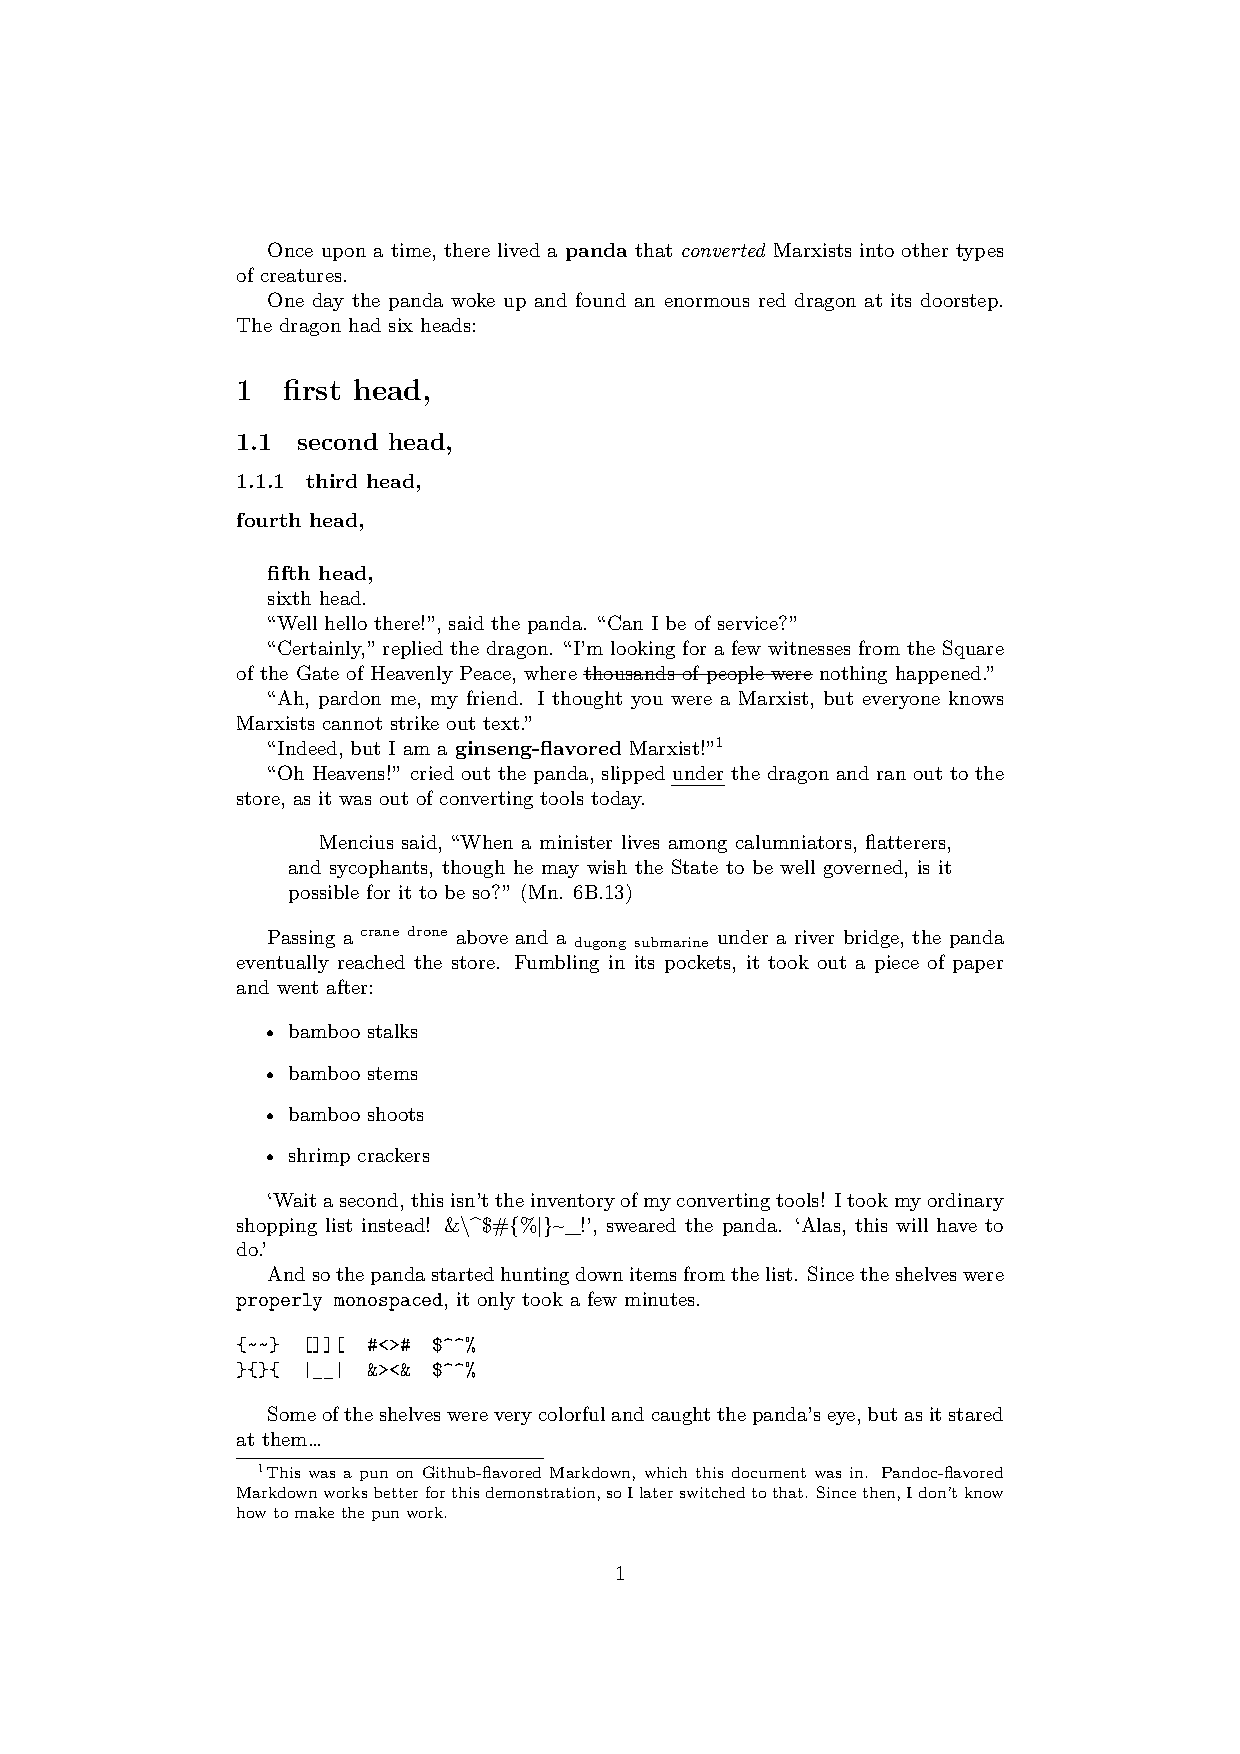
\includegraphics[width=\dimexpr(\textwidth-2\fboxrule-2\fboxsep), trim={4cm 18.1cm 4cm 4cm}, clip]{figures/markdown-panda}}
\caption{An excerpt from the example Markdown document \texttt{panda.md} after it has been typeset using our proof of concept writer.}
\label{fig:example-panda}
\end{figure}

% \includepdf[pages={1}]{pandoc-to-markdown/examples/html-browsers.pdf}

% \begin{figure}[h]
%    \centering
%    \begin{tabular}{@{}c@{\hspace{.5cm}}c@{}}
%      \includegraphics[
%        width=0.6\textwidth,
%        page=1,
%        frame,
%        trim=2cm 2cm 2cm 2cm
%      ]{pandoc-to-markdown/examples/html-browsers.pdf}
%    \end{tabular}
%  \caption{Example page from an \textsc{HTML} document typeset with the proof of concept}
%  \label{fig:html-browsers-typeset}
% \end{figure}

%%%%%%%%%%%%%%%%%%%%%%%%%%%%%%%%%%%%%%%%%%%%%%%%%%%%%%%%%%%%%%%%%%%%%%%%%%%%%%%%
\fi

\chapter{Conclusion}
This thesis demonstrated how the Pandoc utility can be integrated with the Markdown package, resulting in a generic \TeX{} writer that is capable of working with plain \TeX{} and offers ways to directly influence the output of Pandoc.

After a quick introduction, Chapter 2 introduced Pandoc and described its typical usage. It also quickly introduced \TeX{} and the Markdown package, as well as quickly outlining the differences between the elements of Pandoc and Markdown. Chapter 3 then described how the proof of concept for the integration was assembled while showcasing the complete contents of the core files.
\ifexamples
Finally, Chapter 4 showcased the practical use of the proof of concept on a set of example documents.
\fi

\section{Future work}
Some core developers of Pandoc have already expressed prior interest in a plain \TeX{} writer\footnote{\url{https://github.com/jgm/pandoc/issues/1541}} or positive reactions towards the proof of concept\footnote{For example in this thread: \url{https://groups.google.com/g/pandoc-discuss/c/W378Guwz-WA/m/-qaBzU6tAwAJ}}. Given enough time and work, that the showcased proof of concept \TeX{} might eventually mature into a writer worthy of being included in the core distribution of Pandoc. However, there are still many obstacles that would need to be overcome on the way there. In this section, I will try to outline a few of them.

\subsection{Form of the output macros}
Many of the \macro{pandoc...} macros showcased in Chapter 3 were structured after their corresponding \renderer{...} macros instead of the custom writer functions they are related to. This was done mainly because of the difficulty of programming in \TeX{} as compared to Lua. It will be necessary possible to gradually alter the form of the \macro{pandoc...} macros so that their parameters eventually match the parameters of their corresponding custom writer functions. This will require a lot of the transformation logic to be moved from Lua to \TeX{}, which the extensive expl3 interfaces \cite{l3-interfaces} might make relatively painless.

\subsection{Independence from the Markdown package}
The logical next step is to completely remove any dependence of the writer on the Markdown package and reimplement all elements in plain \TeX{}, as well as the \LaTeX{} and Con\TeX{}t layers on top. This might be possible just by looking into what the macros in Markdown expand into.

As for the elements without equivalents in Markdown for which their current macros just output their unchanged parameters, some creativity and/or outreach to the wider \TeX{} community will be necessary.

\subsection{Plain \TeX{} and Con\TeX{}t interfaces}
A quick way to use the proof of concept utilizing a \LaTeX{} package was implemented and demonstrated in this thesis. However, to become a truly generic writer, an interface for plain \TeX{} will have to be developed too. As for other formats like Con\TeX{}t, I believe that the plain \TeX{} interface will be fairly usable in Con\TeX{}t, but it is possible that Con\TeX{}t will offer better, more suitable constructions for the interface.

\subsection{Error handling}
Rewriting a minor parts of the proof of concept, especially in the \LaTeX{} package, in a more robust way would improve the usability of the package in the case that something goes wrong during typesetting.

One example is the line of code in \file{p2md.sty} responsible for running Pandoc. If the command fails, for example because the input file is not available or because its structure is invalid, no output file is produced. This is not communicated to \TeX{} in any way and when \macro{input} called with the output file finally fails, the user is met with a rather cryptic message:

\noindent
\lstset{language=}
\begin{lstlisting}
! I can't find file `man-pandoc.pandoc.tex'.
l.13 \pandocInput[format=man]{files/pandoc.1}
\end{lstlisting}

\noindent
Some error handling mechanism will have to be developed to handle the case in which Pandoc execution fails. As of writing this, I am not aware of any way to check the exit code of a command that runs using shell escape, so this might be a tricky task.

\subsection{Handling of deprecation of classic custom writers}
There are currently two styles of defining custom writers for Pandoc, to which the Pandoc documentation refers to as ``classic'' and ``new''. The main difference between them is that the classic style writer defines its rendering functions on the top level, while in the new style, everything is processed through a top-level function named \texttt{Writer} which contains all the custom writer logic.

For the generic \TeX{} writer, I have decided to go with the classic style. There were multiple reasons for this, the main one being that the classic style is what Pandoc's documentation covers. Another reason is that support for the new style was only introduced in Pandoc 2.18\footnote{The Pandoc documentation actually states that the new style of custom writers was introduced in 2.17.2. This is wrong. No such version was even released, 2.17.1.1 was immediately followed by 2.18.}, which was released in January 2022. Repositories of several high-profile Linux distributions ship versions of Pandoc that are often months older than that. For instance, Fedora 37 released in November 2022 provides only packages with Pandoc 2.14.0.3\footnote{\url{https://packages.fedoraproject.org/pkgs/pandoc/pandoc/fedora-37.html}}, which was released in June 2021. Another example is Ubuntu 22.04 LTS (codenamed ``Jammy Jellyfish''), which, despite being released in April 2022, still ships Pandoc 2.9.2.1\footnote{\url{https://packages.ubuntu.com/jammy/pandoc}} from March 2020.

Unbeknownst to me at the time of writing the proof of concept, classic custom writers were going to be deprecated. According to the discussion on the related pull request,\footnote{\url{https://github.com/jgm/pandoc/pull/8343}} it will still be possible to update a classic writer to a new-style one. However, other breaking changes might still be introduced. As long as the generic \TeX{} writer is an external one instead of being built into Pandoc itself, it will have to deal with this problem in the future versions of Pandoc.

\printbibliography[heading=bibintoc] %% Print the bibliography.

\makeatletter\thesis@blocks@clear\makeatother

\appendix %% Start the appendices.
\chapter{Electronic attachments}
The thesis archive contains \textbf{pandoc-to-markdown.zip}, an archive containing the complete source code of the proof of concept.

\end{document}
